\begin{figure}[htbp]
\centering
%% ── Gemini-generated image version (active) ──────────────────────────────────
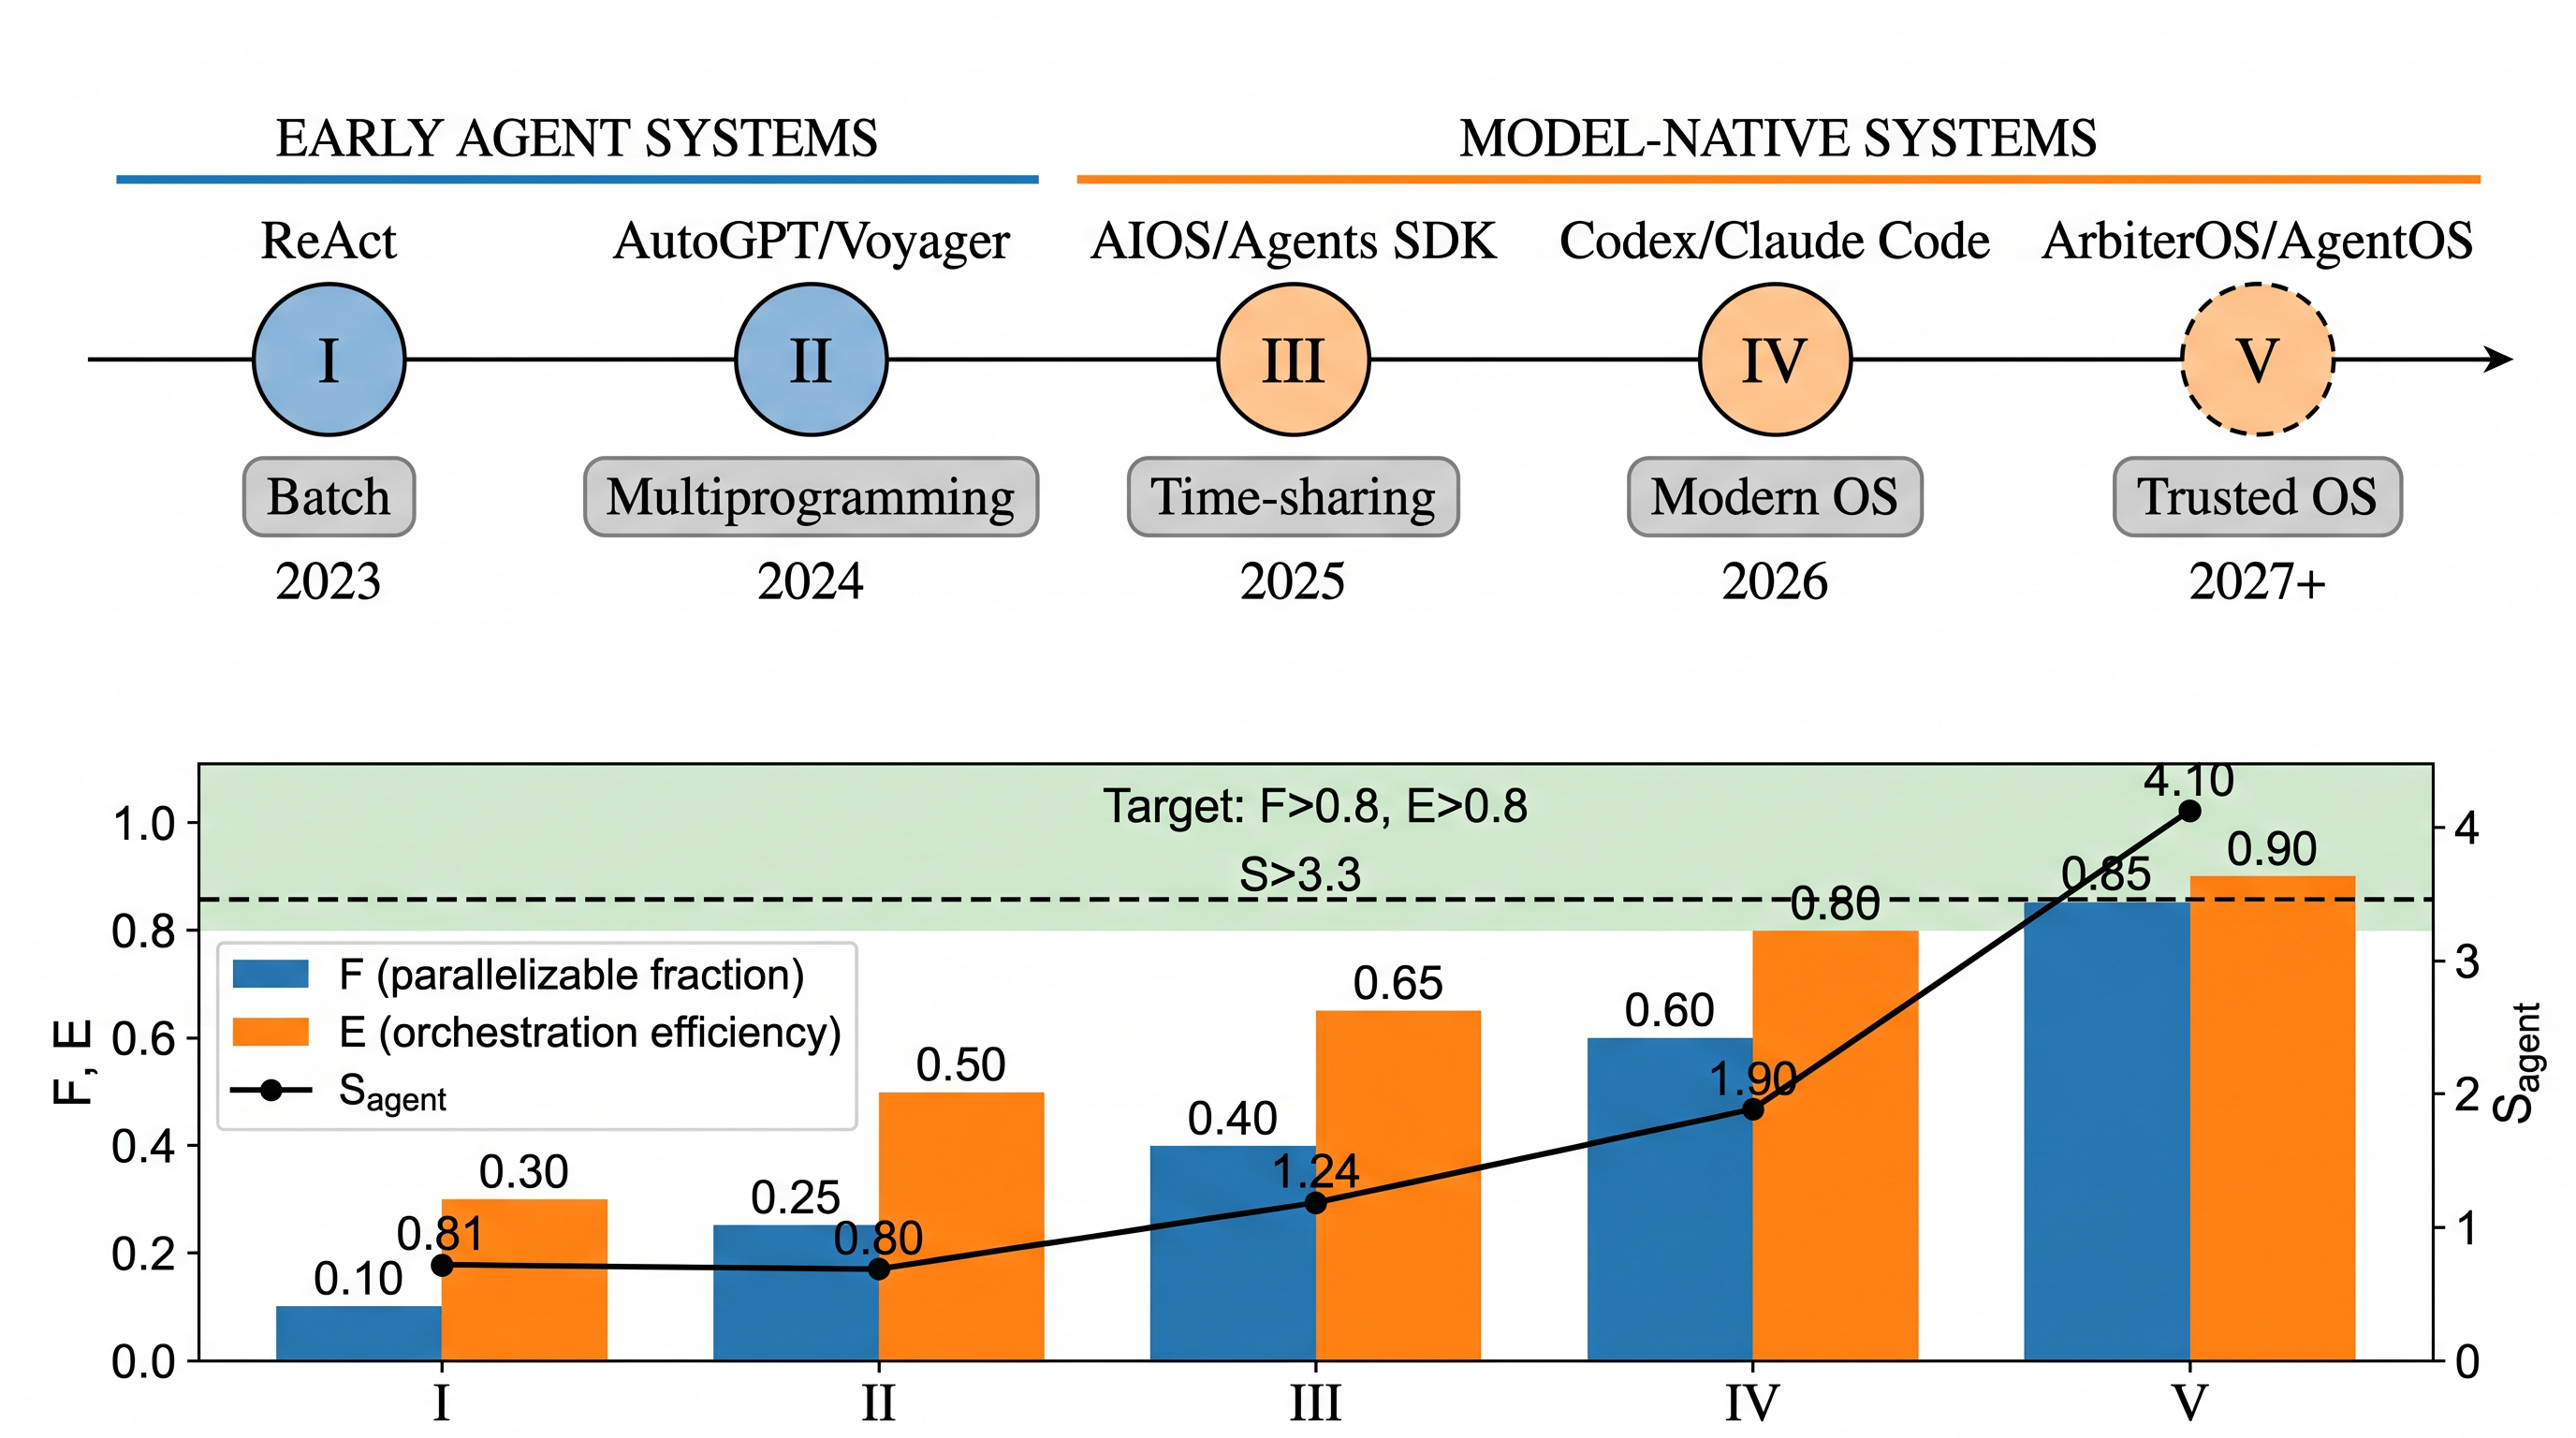
\includegraphics[width=0.95\textwidth]{figures/fig_agent_timeline_gemini.png}
%% ── Original TikZ version (commented out) ────────────────────────────────────
%\resizebox{0.95\textwidth}{!}{%
%\begin{tikzpicture}[
%    font=\sffamily,
%    >=Stealth,
%    milestone/.style={
%        circle,
%        minimum size=10mm,
%        inner sep=0pt,
%        line width=0.9pt,
%        font=\small\bfseries
%    },
%    early/.style={
%        milestone,
%        fill=softBlue,
%        draw=timelineBlue,
%        text=timelineBlue
%    },
%    native/.style={
%        milestone,
%        fill=softOrange,
%        draw=timelineOrange,
%        text=timelineOrange
%    },
%    future/.style={
%        native,
%        dashed
%    },
%    framework/.style={
%        align=center,
%        text width=29mm,
%        font=\small\bfseries,
%        text=timelineDark
%    },
%    oschip/.style={
%        rounded corners=2.5pt,
%        fill=softGray,
%        draw=timelineGray!65,
%        line width=0.45pt,
%        inner xsep=5pt,
%        inner ysep=2.6pt,
%        font=\scriptsize\itshape,
%        text=timelineDark,
%        align=center
%    },
%    year/.style={
%        font=\scriptsize\bfseries,
%        text=timelineGray!85!black
%    },
%    phase/.style={
%        font=\scriptsize\bfseries,
%        text=timelineDark
%    },
%    flow/.style={
%        -{Stealth[length=2.4mm,width=1.6mm]},
%        draw=timelineGray,
%        line width=0.95pt
%    }
%]

% Milestone nodes
%\node[early]  (g1) at (0.0,  0) {I};
%\node[early]  (g2) at (3.4,  0) {II};
%\node[native] (g3) at (6.8,  0) {III};
%\node[native] (g4) at (10.2, 0) {IV};
%\node[future] (g5) at (13.6, 0) {V};

% Evolution arrows
%\draw[flow] (g1.east) -- (g2.west);
%\draw[flow] (g2.east) -- (g3.west);
%\draw[flow] (g3.east) -- (g4.west);
%\draw[flow] (g4.east) -- (g5.west);

% Framework names
%\node[framework, above=5mm of g1] {ReAct};
%\node[framework, above=5mm of g2] {AutoGPT\\Voyager};
%\node[framework, above=5mm of g3] {AIOS\\Agents SDK};
%\node[framework, above=5mm of g4] {Codex\\Claude Code};
%\node[framework, above=5mm of g5] {ArbiterOS\\AgentOS};

% Operating-system analogies
%\node[oschip, below=8mm of g1] (o1) {Batch};
%\node[oschip, below=8mm of g2] (o2) {Multiprogramming};
%\node[oschip, below=8mm of g3] (o3) {Time-sharing};
%\node[oschip, below=8mm of g4] (o4) {Modern OS};
%\node[oschip, below=8mm of g5] (o5) {Trusted OS};

% Years
%\node[year, below=4mm of o1] {2023};
%\node[year, below=4mm of o2] {2024};
%\node[year, below=4mm of o3] {2025};
%\node[year, below=4mm of o4] {2026};
%\node[year, below=4mm of o5] {2027+};

% Phase headers
%\draw[timelineBlue, line width=0.95pt]
%    (-0.45, 2.28) -- (4.65, 2.28);
%\node[phase, text=timelineBlue]
%    at (2.10, 2.55) {EARLY AGENT SYSTEMS};

%\draw[timelineOrange, line width=0.95pt]
%    (5.95, 2.28) -- (14.05, 2.28);
%\node[phase, text=timelineOrange]
%    at (10.00, 2.55) {MODEL-NATIVE SYSTEMS};

%% ===========================================================
%% BOTTOM ROW: Quantitative F / E / S_agent chart (pgfplots)
%% ===========================================================
%% S_agent values computed via Law III:  S = 1/((1-F)+F/(N*E))
%%   Gen I:   N=1,  F=0.10, E=0.30 => S=0.81
%%   Gen II:  N=1,  F=0.25, E=0.50 => S=0.80
%%   Gen III: N=3,  F=0.40, E=0.65 => S=1.24
%%   Gen IV:  N=6,  F=0.60, E=0.80 => S=1.90
%%   Gen V:   N=10, F=0.85, E=0.90 => S=4.10

% ---- Left axis: F and E bars ----
%\begin{axis}[
%    name=barchart,
%    at={(-1.2,-8.0)},
%    anchor=north west,
%    width=15.6cm,
%    height=5.8cm,
%    ybar,
%    bar width=7pt,
%    ymin=0, ymax=1.08,
%    xmin=-0.5, xmax=4.5,
%    xtick={0,1,2,3,4},
%    xticklabels={I, II, III, IV, V},
%    xticklabel style={font=\sffamily\small\bfseries, color=timelineDark},
%    ytick={0,0.2,0.4,0.6,0.8,1.0},
%    yticklabels={0, 0.2, 0.4, 0.6, 0.8, 1.0},
%    yticklabel style={font=\sffamily\scriptsize, color=timelineDark},
%    ylabel={\small $F$,\; $E$},
%    ylabel style={font=\sffamily\small, color=timelineDark, at={(0.06,0.5)}},
%    axis y line*=left,
%    axis x line*=bottom,
%    enlarge x limits=0.15,
%    legend style={
%        at={(0.02,0.55)},
%        anchor=north west,
%        font=\sffamily\scriptsize,
%        draw=timelineGray!50,
%        fill=white,
%        fill opacity=0.9,
%        text opacity=1,
%        row sep=1pt,
%        /tikz/every even column/.append style={column sep=4pt}
%    },
%    tick style={draw=none},
%    major grid style={draw=timelineGray!20, line width=0.3pt},
%    ymajorgrids=true,
%    clip=false,
%]

% --- Target zone (F>0.8 and E>0.8 shaded region) ---
%\fill[green!12, opacity=0.5]
%    (axis cs:-0.5,0.8) rectangle (axis cs:4.5,1.08);
%\draw[green!50!black, densely dashed, line width=0.5pt]
%    (axis cs:-0.5,0.8) -- (axis cs:4.5,0.8);
% Label at top-right of green band, above the bars
%\node[font=\sffamily\tiny\itshape, text=green!40!black, anchor=north east]
%    at (axis cs:4.5,1.08) {Target: $F{>}0.8,\;E{>}0.8$};

% --- F bars (parallelizable fraction) ---
%\addplot[
%    fill=timelineBlue!55,
%    draw=timelineBlue,
%    line width=0.4pt
%] coordinates {
%    (0, 0.10)
%    (1, 0.25)
%    (2, 0.40)
%    (3, 0.60)
%    (4, 0.85)
%};
%\addlegendentry{$F$ (parallelizable fraction)}

% --- E bars (orchestration efficiency) ---
%\addplot[
%    fill=timelineOrange!55,
%    draw=timelineOrange,
%    line width=0.4pt
%] coordinates {
%    (0, 0.30)
%    (1, 0.50)
%    (2, 0.65)
%    (3, 0.80)
%    (4, 0.90)
%};
%\addlegendentry{$E$ (orchestration efficiency)}

%\end{axis}

% ---- Right axis: S_agent line ----
%\begin{axis}[
%    at={(barchart.south east)},
%    anchor=south east,
%    width=15.6cm,
%    height=5.8cm,
%    ymin=0, ymax=4.5,
%    xmin=-0.5, xmax=4.5,
%    xtick=\empty,
%    ytick={0,1,2,3,4},
%    yticklabels={$0$,$1$,$2$,$3$,$4$},
%    yticklabel style={font=\sffamily\scriptsize, color=timelineDark},
%    ylabel={\small $S_{\mathrm{agent}}$},
%    ylabel style={font=\sffamily\small, color=timelineDark, at={(0.96,0.5)}},
%    axis y line*=right,
%    axis x line=none,
%    enlarge x limits=0.15,
%    clip=false,
%    legend style={
%        at={(0.98,0.98)},
%        anchor=north east,
%        font=\sffamily\scriptsize,
%        draw=timelineGray!50,
%        fill=white,
%        fill opacity=0.9,
%        text opacity=1,
%        row sep=1pt
%    },
%]

% --- S_agent smooth line ---
%\addplot[
%    thick,
%    timelineDark,
%    mark=*,
%    mark size=2.5pt,
%    mark options={fill=timelineDark},
%    line width=1.1pt,
%    smooth
%] coordinates {
%    (0, 0.81)
%    (1, 0.80)
%    (2, 1.24)
%    (3, 1.90)
%    (4, 4.10)
%};
%\addlegendentry{$S_{\mathrm{agent}}$}

% --- S_agent value labels ---
%\node[font=\sffamily\tiny\bfseries, text=timelineDark, anchor=south]
%    at (axis cs:0,0.81) {0.81};
%\node[font=\sffamily\tiny\bfseries, text=timelineDark, anchor=south]
%    at (axis cs:1,0.80) {0.80};
%\node[font=\sffamily\tiny\bfseries, text=timelineDark, anchor=south]
%    at (axis cs:2,1.24) {1.24};
%\node[font=\sffamily\tiny\bfseries, text=timelineDark, anchor=south]
%    at (axis cs:3,1.90) {1.90};
%\node[font=\sffamily\tiny\bfseries, text=timelineDark, anchor=south]
%    at (axis cs:4,4.10) {4.10};

% --- Target S_agent dashed line at S=3.3 ---
%\draw[timelineDark, densely dotted, line width=0.6pt]
%    (axis cs:-0.5,3.3) -- (axis cs:4.5,3.3);
%\node[font=\sffamily\tiny\itshape, text=timelineDark, anchor=east]
%    at (axis cs:4.5,3.5) {$S{>}3.3$};

%\end{axis}

%\end{tikzpicture}}% end resizebox
\caption{Agent framework evolution from single-turn reasoning to model-native operating systems.
\textbf{Top:} representative frameworks with analogous OS milestones.
\textbf{Bottom:} quantitative trajectory of parallelizable fraction ($F$), orchestration efficiency ($E$), and agent speedup ($S_{\mathrm{agent}}$) per Law~III; green band marks the target regime ($F{>}0.8,\;E{>}0.8$).}
\label{fig_agent_timeline}
\end{figure}
